\section{Chapter 10 -- Our Star}
\subsection{A Closer Look at the Sun}
\subsubsection{History}
Our first views of the sun were that it was a ball of fire. In the $19^{th}$ century we had found the Sun's radius and distance and found that its energy could not have come from burning fuels or other chemical processes.

The first real idea was that the Sun generates energy by slowly contracting in size through \textbf{gravitational contraction}. Gravitational potential energy is converted into thermal energy as mass moves inward. This would keep the inside of the Sun hot. The amount of contraction required would be small enough to go unnoticed until the $19^{th}$ century. This theory shows that the Sun could continue contracting for 25 million years. The problem: geologists had already calculated the earth's age as much higher than that.

The next idea was based on Einstien's theory of relativity ($E=mc^2$). Calculations showed that the Sun had enough mass to shine for billions of years. This explained where sunlight came from, but not the thermal energy. Eventually in the  1930's the discovery of nuclear fusion was found and we use that to explain where thermal energy comes from.

\subsubsection{Nuclear Fusion}
Nuclear fusion requires very high temperature and density to start. This started in the sun through gravitational contraction. The sun was formed from a collapsing gas cloud. This released gravitational potential energy raisin the core temperature. This continued to happen until sustained nuclear fusion started.

The sun has a fairly steady size and energy today because it has reached equilibrium. \textbf{Gravitaitonal Equilibrium} is the balance between the outward push of hot internal gases trying to escape and the inward push of gravity. This allows the sun to have a steady size. This also means that \textbf{pressure increases with depth} in the sun. \textbf{Energy Balance} is the balance between the rate of fusion and the rate of energy being released from the Sun's core into space.

\subsubsection{Structure}
The sun is essentially a ball of plasma (gas in which atoms are ionized) which moves like a gas, but also reacts to magnetic fields.

Basic Properties:\\
\begin{tabular}{|c|c|}
\hline
Radius (R Sun ) & 696,000 km (about 109 times the radius of Earth)\\
\hline
Mass (M Sun )  & 2 ϫ 10 30 kg (about 300,000 times the mass of Earth)\\
\hline
Luminosity/Power Output (L Sun ) & 3.8 ϫ 10 26 watts\\
\hline
Composition (by percentage of mass) & 70\% hydrogen, 28\% helium,2\% heavier elements\\
\hline
Rotation rate & 25 days (equator) to 30 days (poles)\\
\hline
Surface temperature & 5800 K (average); 4000 K(sunspots)\\
\hline
Core temperature & 15 million K\\
\hline
\end{tabular}

Layers (outside in):
\begin{itemize}
\item Solar wind
\item Corona
\item Chromosphere
\item Photosphere
\item Convection zone
\item Radiation zone
\item Core
\end{itemize}
\textbf{Solar Winds} is a stream of charged particles blown outward from the Sun. These help shape the magnetospheres of planets and the tails of comets.

\textbf{Corona} is suprisingly hot (1 million K) and emits the most X-ray radiation, the density is very low

\textbf{Chromosphere} is much cooler here (10,000 K), radiates UV radiation

\textbf{Photosphere} temperature is 6,000K, surface churns like boiling water, home of sunspots and intense magnetic fields

\textbf{Convection Zone} region of hot gas rising and cool gas sinking caused by energy from the core rising to the surface (called convection, duh)

\textbf{Radiation Zone} less turbulent than the convection zone, energy moves outwards as photons instead of hot gas, temperature rises to 10 million K, shit ton of X-ray radiation

\textbf{Core} where nuclear fusion is making energy, temperature 15 million K, density 100 that of water, pressure 200 billion times earth's surface, energy takes hundreds of thousands of years to get to the surface

\subsection{Nuclear Fusion in the Sun}
Note nuclear fusion (the Sun) $\not =$ nuclear fision (nuclear reactor).

Within the Sun's core there is a soup of hot fas funn of psitively charged atom nuclei flying about. When these collide (most of the time electormagnetic forces deflect them) they stick together to form a heavier nucleus. This is caused by \textbf{strong force} (binds protons and neutrons together) overriding the electromagnetic deflection force. It's only strong enough to do this at very small distances which happens due to the high speed of the particles (which is in turn caused by the high temperature which is caused by the high pressure which is caused by high gravitational force which is caused by large mass).

This is explained by the \textbf{Ideal Gas Law} \[ P = nkT \] where P is the pressure, n is number density (particles per volume), T is temperature, and k is \textbf{Boltzmann constant} $=1.38 \times 10^{-23}$ joule/K

\subsubsection{Proton-Proton Chain}
Most hydrogen comes in the form of a single proton, but we need to fuse it into a helium atom which is two protons and two neutrons. So what we have to do is fuse four hydrogen atoms into one helium atom. This is through a sequence of events called the \textbf{proton-proton chain}.
\begin{enumerate}
\item Two protons fuse to make a deuterium nucleus (1 proton and 1 neutron). This step occurs twice
\item The deuterium nucleus and a proton fuse to make a nucleus of helium-3 (2 protons, 1 neutron). This step occurs twice
\item Two helium-3 nuclei fuse to form helium-4 (2 protons, 2 neutrons), releasing two excess protons in the process.
\end{enumerate}
In total four protons collide to make a helium atom, two positrons, and two neutrinos.

\subsubsection{Solar Thermostat}
Life on earth relies on the Sun's steady fusion rate. If we were to increase the core's temperature slightly, this would cause an increase in fusion rate. The increased fusion rate would make more energy, but energy moves very slowly through the sun so it would get bottled up in the core. This would increase the core pressure to exceed the balancing force of gravity so the core would expand and cool. Cooling lowers the fusion rate and equilibrium is reached again.

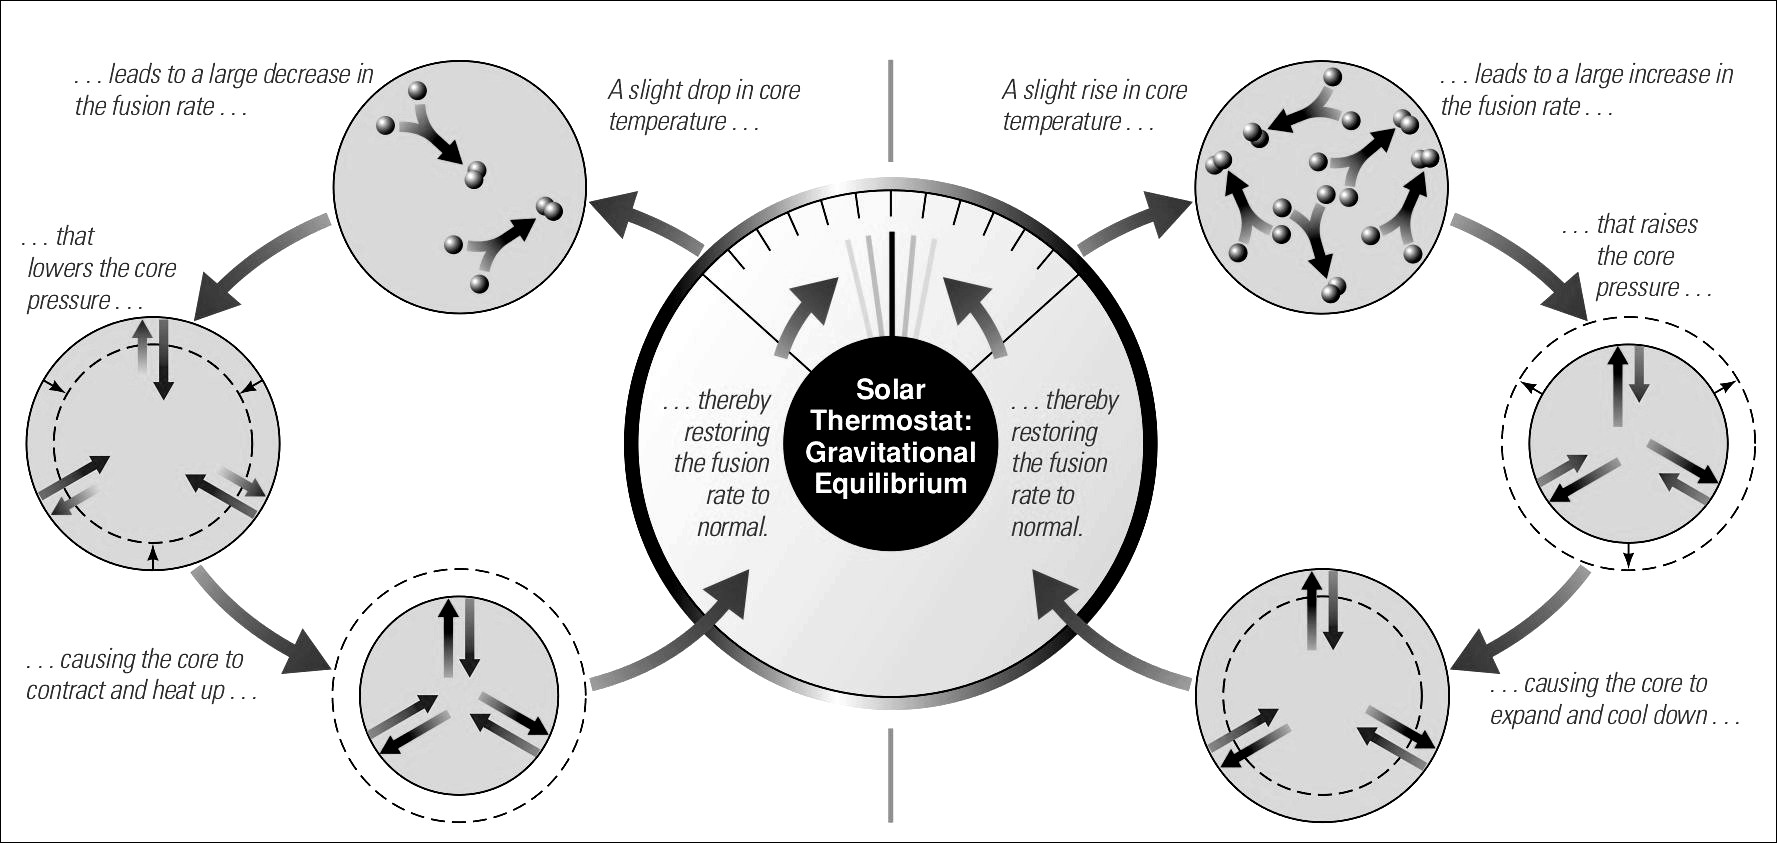
\includegraphics[width=\textwidth]{solarThermostat}

\subsubsection{Path of Energy Through the Sun}
Energy starts as photons in the Sun's core. They zigzag at the speed of light so it takes them a while to get out. In the dense interior a photon can only ravel a fraction of a millimeter before it collides with electron and gets deflected in a new direction causing its zigzag path. Eventually it makes its way through the core and radiation zone into the convection zone where the temperature drops to 2 million K and the photon is absorved into cooler solar plasma. This creates the convection that happens in the convection zone. Eventually it rises to the top and enters the photosphere. Here the density is low enough that photons can escape into space as sunlight.

How do we know about the interior of a star:
\begin{itemize}
\item Mathematical models: based on laws of physics and observed properties
\item Solar Vibrations: the Sun's surface vibrates like with earthquakes which we can see in Doppler Shifts.
\item Solar Neutrinos: these are formed during nuclear fusion, these can pass through almost anything without reacting (including the Sun's layers), so we can see whats going on right now (well, 8 minutes ago)
\begin{itemize}
\item these fuckers are hard to catch, need detectors deep in mines
\item initially we only caught a third of what we expected (solar neutrino problem) due to neutrinos changing properties during their journey (electron neutrino, muon neutrino, or tau neutrino)
\end{itemize}
\end{itemize}

\subsection{The Sun-Earth Connection}
\subsubsection{Sunspots and Magnetic Fields}
\textbf{Sunspots} are dark spots on the sun where things are cooler. They are formed when magnetic fields keep hot gas from entering a section of the photosphere. Magnetic fields can alter the energy levels of atoms (Zeeman effect), mucking with their spectral lines. The particles in solar plasma move along magnetic lines (usually spiraling along them).

Sunspots form where magnetic fields extend from the Sun's interior. The magnetic lines there are strong enough to suppress convection making the spot cool. They usually last a few weeks until their magnetic fields weaken. Sunspots tend to appear in pairs connected by a magnetic loop. Gas getting trapped in these loops makes \textbf{solar prominences}.

\subsubsection{Solar Storms}
These are sudden changes in the Sun's magnetic fields. The most dramatic example is \textbf{solar flares} which send bursts of X rays and fast moving particles into space. Flares tend to happen near sunspots. The current theory is that solar flares are caused when magnetic fields become so twisted they cannot bear the tension and snap into a better shape.

\subsubsection{Heating the Chromosphere and Corona}
Some weird shit goes down on the sun where its atmosphere gets hotter the farther you go out. The current theory is that magnetic fields carry energy upward to heat the chromosphere and corona.

The churning that happens in the convection zone probably shakes with tightly wound magnetic lines which carry this energy into the atmosphere and deposit it as heat.

Its very hard to investigate this because the solar atmosphere is not dense enough to see at that point (except during an eclipse). We can watch them through X-rays and UV rays.

In X-ray images of the chronosphere:
\begin{itemize}
\item bright spots is where hot gas is trapped below a sunspot where magnetic lines loop back to the Sun
\item dull spots (\textbf{coronal holes}) are under magnetic lines that escape into space
\item the stuff blown out by flares are huge bubbles called \textbf{coronal mass ejections}
\begin{itemize}
\item have strong magnetic fields
\item causes auroras
\item fuck with satellites
\end{itemize}
\end{itemize}

\subsubsection{Solar Cycles}
Sunspots have a 11 year cycle. The solar maximum has most sunspots and solar minimum has fewest. At each solar maximum the Sun's magnetic fields start to flip. This is because all magnetic lines connecting pairs of sunspots point the same direction. This means that magnetic fields have a 22 year cycle.
